\documentclass[11pt,a4paper]{article}

\usepackage[margin=25mm]{geometry}
\usepackage[T1]{fontenc}
\usepackage{lmodern}
\usepackage{microtype}
\usepackage{booktabs}
\usepackage{longtable}
\usepackage{tabularx}
\usepackage{siunitx}
\usepackage{graphicx}
\usepackage{float}
\usepackage{listings}
\usepackage{xcolor}
\usepackage{enumitem}
\usepackage{hyperref}

\sisetup{group-separator={,},group-minimum-digits=4}
\hypersetup{
  colorlinks=true,
  linkcolor=blue!50!black,
  citecolor=blue!50!black,
  urlcolor=blue!50!black,
  pdftitle={Instance-space analysis of the H-ODBRP},
  pdfauthor={Michell Queiroz}
}
\newcommand{\tagopen}[1][]{\textbf{[OPEN\ifx\relax#1\relax\else-#1\fi]}}
\newcommand{\tagprop}{\textbf{[PROPOSED]}}
\newcommand{\tagdone}{\textbf{[DECIDED]}}
\newcommand{\sourcepath}[1]{{\small\protect\path{#1}}}
\setlist{nosep,leftmargin=*}
\lstset{
  basicstyle=\ttfamily\small,
  columns=fullflexible,
  breaklines=true,
  frame=single,
  keepspaces=true
}

\title{Instance-Space Analysis for the Heterogeneous\\On-Demand Bus Routing Problem}
\author{Michell Queiroz}
\date{Draft based on the source set updated 29 October 2026}

\begin{document}
\maketitle

\begin{abstract}
This report records the design, implementation, and preliminary evidence for an
instance-space analysis (ISA) of the static heterogeneous on-demand bus routing
problem (H-ODBRP). The study uses simulated annealing (SA) and a greedy
construction (GR) as the current comparison pair. A pilot of 24 generated
instances paired with three fleets produced 72 solver cases. SA was better on
70 of 72 cases; the two-level pilot still has a gap along the time-window
dimension. A seed defect was identified and fixed, and the reported count of
distinct mean OD distances rose from 6 to 24. A rewritten exact model and a
checker replace an original model that disagreed with the heuristic rules in
9 of 11 scenarios. Full-set generation is not yet established: the station
matrix job, memory sizing, a third algorithm, and several design choices remain
\tagopen. The proposed full design uses a Latin hypercube over the Capital
Region of Denmark, excluding Bornholm, and grows in batches as the instance
space expands.
\end{abstract}

\section{Summary}

The study asks how instance characteristics relate to the performance of
algorithms for the static H-ODBRP. Instances are described by demand, time
window, fleet, and network features, then projected into a low-dimensional
instance space. SA and GR form the present performance matrix. The exact
Gurobi model is reserved for validation on very small cases; a MIP-based
large-neighbourhood matheuristic is intended to show where SA can improve, not
to act as a third ISA algorithm.

Work completed includes a 72-case Copenhagen pilot, a correction to request
seeding, a network cut-out for Bornholm, a nearest-node cache, solver input
fixes, an exact-model checker, a rewritten exact model, and HPC job scripts.
The pilot suggests that SA is usually better than GR: SA wins on 70 of 72
cases. GR is competitive in a narrow corner: tight time windows and the
smallest pilot fleet. The pilot projection retains a gap associated with the
two time-window settings. The available feature CSVs do not independently
reproduce the documented pre-fix count of six distinct mean OD distances; the
post-fix CSV does contain 24.

The proposed full design covers 100--1000 requests in a two-hour period and
draws instance settings and fleets using Latin hypercubes. The region, period,
and ranges remain \tagprop; the author has the final decision. The new exact
model agrees with the heuristic feasibility checks in all 11 tested
scenarios, while the original model disagreed in 9. On rerun, the new model
proved the five-request case in 2.5 seconds, but had a 25\% gap at the limit
for 10 requests and did not prove the 15-request case.

The full instance set is still blocked by unresolved generation cost and
memory questions, an unrun station-matrix build, and the missing shared-matrix
feature step. Other open work includes the third ISA algorithm, the
matheuristic HPC test, solver resource sizing, and final design choices. These
results are preliminary, and the one-sided SA--GR result must be tested on the
wide design.

\section{Study design}

\subsection{Network, period, and instance settings}

The study network is the whole Capital Region of Denmark without Bornholm.
Instances use a two-hour planning period beginning between 12:00 and 19:30.
The current design draws 50--500 requests per hour (100--1000 in each
instance). All instance ranges below are the present values in
\sourcepath{isa_set/design.json}; the settings document describes them as
\tagprop unless stated otherwise.

\begin{longtable}{@{}p{0.19\linewidth}p{0.22\linewidth}p{0.32\linewidth}p{0.18\linewidth}@{}}
\caption{Study settings, comparison with the earlier papers, and current status. [H] and [P] refer to the two papers in \cite{queiroz2026evaluation,queiroz2026parallel}.}\\
\toprule
Setting & Study range & Paper range & Status\\
\midrule
\endfirsthead
\toprule
Setting & Study range & Paper range & Status\\
\midrule
\endhead
Network & Capital Region, excluding Bornholm & Chicago [H]; city scenarios [P] & \tagprop\\
Planning period & 2 hours & 1 hour [H]; 2--7 hours [P] & \tagprop\\
Start time & 12:00--19:30 & Commuting and event windows [P] & \tagprop\\
Requests & 50--500 per hour (100--1000 per instance) & 300--3000 per hour [H]; 5000--20000 per scenario [P] & \tagprop; \tagopen[S1]\\
Peak spread & 10--60 min standard deviation & About 15 min plus 40\% uniform in one [P] scenario & \tagprop\\
Urgency mean & 5--40 min & 5, 10, 15, 30 min [H] & \tagprop\\
Urgency standard deviation & 1--10 min & 0, 5, 10 min [H] & \tagprop\\
Arrival slack & 5--60 min & Not varied & \tagprop\\
Maximum walking time & 550--600 s & Generator default; 550--600 s in earlier settings & \tagprop; \tagopen[S2]\\
Walking speed & 1.38889 m/s & Same & \tagprop\\
Direct trip time & 300--3600 s & Same lower bound; study upper bound raised for suburbs & \tagprop\\
Vehicle speed & 20 km/h & Same & \tagprop\\
Fleet size & 5--40\% of requests & 10--21\% [H] & \tagprop\\
Eight-seat share & 0--100\%; remainder four-seat & Four- and eight-seat mix performed well [H] & \tagprop\\
Fleet draws & 3 per generated instance & Fleet fixed per instance [P] & \tagprop\\
Depot & One station unused by requests, selected after generation & Several depots [H] & \tagdone; \tagopen[S3]\\
\bottomrule
\end{longtable}

The network build produced 3515 stations and no station on Bornholm. The
station-to-station travel-time matrix is intended to be computed once for the
network, in a separate HPC job. The number of batches is not fixed: batches of
100 are proposed until fewer than about 5\% of new instances are far from
existing ones, or a cap is reached. The cap remains \tagopen[S4].

\subsection{Axes of the instance space}

The feature list confirms 18 features for the static ISA. The last three
features in the list are dynamic-only; the two network features at the end are
not implemented for this study.

\begin{longtable}{@{}p{0.30\linewidth}p{0.63\linewidth}@{}}
\caption{Static ISA features and their short definitions.}\\
\toprule
Feature & Definition\\
\midrule
\endfirsthead
\toprule
Feature & Definition\\
\midrule
\endhead
\texttt{n\_requests} & Number of requests.\\
\texttt{demand\_density} & Requests per square kilometre of service area.\\
\texttt{spatial\_cluster\_coeff} & Clark--Evans nearest-neighbour ratio for request origins.\\
\texttt{od\_distance\_mean} & Mean origin--destination driving distance.\\
\texttt{od\_distance\_std} & Standard deviation of origin--destination driving distance.\\
\texttt{tw\_width\_mean} & Mean time-window width.\\
\texttt{tw\_width\_std} & Standard deviation of time-window width.\\
\texttt{tw\_overlap\_ratio} & Fraction of request pairs with overlapping time windows.\\
\texttt{tight\_tw\_fraction} & Fraction of requests with window width below 20 minutes.\\
\texttt{tw\_tightness\_factor} & Mean time-window width divided by minimum trip time.\\
\texttt{fleet\_size} & Number of vehicles relative to request count.\\
\texttt{capacity\_cv} & Standard deviation of vehicle capacities divided by their mean.\\
\texttt{fleet\_utilization\_ratio} & Total fleet capacity divided by request count.\\
\texttt{request\_vehicle\_ratio} & Request count divided by fleet size.\\
\texttt{station\_density} & Bus stops per square kilometre.\\
\texttt{bsa\_flexibility} & Mean available pick-up or drop-off stops per passenger.\\
\texttt{avg\_station\_degree} & Mean degree of bus stops in the road graph.\\
\texttt{coverage\_ratio} & Fraction of the service area within 500 m of a bus stop.\\
\bottomrule
\end{longtable}

\subsection{Fleets, algorithms, and performance}

Each generated request instance is paired with three fleets. Fleet size is
drawn from 5--40\% of requests; the eight-seat share is drawn from 0--100\%,
with the remainder in four-seat vehicles. The depot is selected after
generation at a station not used by a request.

The objective is total passenger ride time plus four times direct travel time
for each request sent to a third party. Operator cost is not in the objective;
vehicle use and driving time may be recorded as post-hoc measures.

The performance matrix currently compares SA with GR. The exact Gurobi model
is used only for validation on 5--15 requests. A third ISA algorithm is
\tagopen: the options are another SA configuration or a max-ALNS variant. The
matheuristic is not a candidate ISA algorithm.

\section{What was implemented}

\subsection{Generator changes}

\begin{longtable}{@{}p{0.20\linewidth}p{0.19\linewidth}p{0.24\linewidth}p{0.22\linewidth}@{}}
\caption{ISA-specific generator changes against the original REQreate.}\\
\toprule
Change & File(s) & Why & Effect\\
\midrule
\endfirsthead
\toprule
Change & File(s) & Why & Effect\\
\midrule
\endhead
Config-dependent request seeds & \sourcepath{REQreate/passenger_requests.py} & All configs previously reused locations. & 24 distinct \texttt{od\_distance\_mean} values after the fix; pre-fix count is not reproduced by available CSVs.\\
Place exclusions & \sourcepath{retrieve_network.py}, \sourcepath{input_json.py}, \sourcepath{schema/config.schema.json}, \sourcepath{cli.py} & Exclude the island of Bornholm from the region polygon. & The network build reported no Bornholm stations.\\
Polygon-scoped points of interest & \sourcepath{osm_features.py}, station, school, and hospital retrieval & Place-name lookup had allowed an outside station to leak in. & 3515 stations; none on Bornholm.\\
Cached nearest-node index & \sourcepath{REQreate/nearest.py}, \sourcepath{passenger_requests.py}, \sourcepath{network_class.py} & Nearest-node calls repeatedly converted the full graph. & Unit test matches OSMnx on 30 random points. Profile timings improved after the cache; memory measurement is suspect.\\
ISA feature export & \sourcepath{REQreate/isa_features_hook.py} & Record one feature row per generated instance. & Feature errors are logged without stopping generation.\\
Station-matrix chunked searches & \sourcepath{REQreate/compute_distance_matrix.py}, \sourcepath{isa_set/station_matrix.py} & Avoid a full graph row cache and Python all-pairs loop. & Same whole-second values in a unit test; separate HPC run remains \tagopen.\\
Pilot v2 sampling & \sourcepath{pilot/run_pilot.py} & Use a real 7:30 peak, replicas, and three fleet sizes. & Replaces the earlier flattened demand peak.\\
\bottomrule
\end{longtable}

\subsection{Solver changes}

\begin{itemize}
\item The \sourcepath{--greedy_only} option runs GR from the SA binary, avoiding
  a separate code base.
\item The solver now reads travel-time matrices as directed (row = from,
  column = to); it no longer symmetrises them.
\item The type-3 request reader converts walking distance in metres to seconds
  using the walking speed.
\item The station limit was raised from 2000 to 4000 for the 3515-station
  region. This ODBRP\_P change is uncommitted; the author must commit it
  \tagopen[A4].
\item The original IP model was replaced by
  \sourcepath{model/MDHODBRP_model_v2.cpp}. Its checker,
  \sourcepath{model/check_model.py}, tests hand-made routes without a Gurobi
  dependency.
\item A MIP-based LNS matheuristic re-solves parts of SA solutions using v2.
  Its HPC run is \tagopen[A2].
\end{itemize}

\subsection{HPC tooling}

The set tooling includes \sourcepath{isa_set/design.json} for ranges,
\sourcepath{isa_set/make_batch.py} for Latin-hypercube batches,
single-core-per-config generation scripts, and a profiling script. Pilot
solver job generation and result collection are provided by
\sourcepath{pilot/make_solver_jobs.py} and
\sourcepath{pilot/collect_results.py}. The station-matrix implementation is
written, but its HPC run and measured resource profile remain \tagopen[G3].

\section{Tests and preliminary results}

\subsection{Pilot instance space and SA versus GR}

The pilot contains 12 configurations with two replicas (24 request instances),
each paired with three fleets (72 solver cases). It uses 200, 500, or 1000
requests; peak standard deviations of 15 or 30 minutes; tight or loose
time-window settings; and fleets at 10\%, 20\%, or 30\% of request count.
The instance-space plot shows the two time-window groups and colours cases by
the SA-to-GR ratio. The documented gap is tied to having only two levels on
this axis; the full design uses continuous ranges \tagprop.

\begin{figure}[H]
\centering
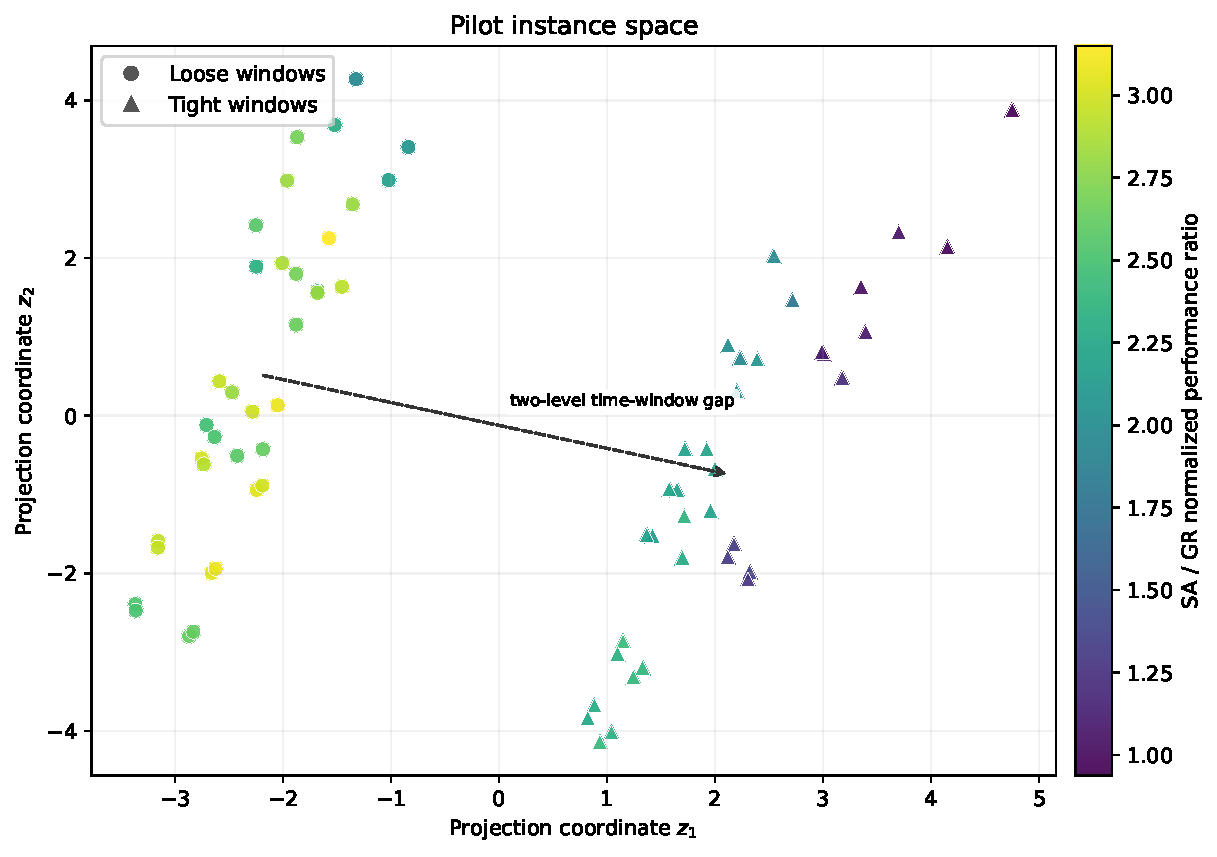
\includegraphics[width=0.88\linewidth]{figures/instance_space.pdf}
\caption{Pilot projection \texttt{z1}--\texttt{z2}. Colour is the SA/GR ratio of
the normalized performance values (above 1 favours SA); marker shape separates
tight and loose time windows. The arrow marks their centroid separation and
the two-level time-window gap. Data: \sourcepath{pilot/work/results/instance_space.csv}
and \sourcepath{pilot/work/results/perf_matrix.csv}.}
\end{figure}

Across all cases, SA is better on 70 of 72. GR is competitive only for tight
windows with the smallest fleet (8 of 72). This one-sided result may make the
pilot's algorithm-selection story thin. Whether it persists in the wide design
is \tagopen[A6].

\begin{figure}[H]
\centering
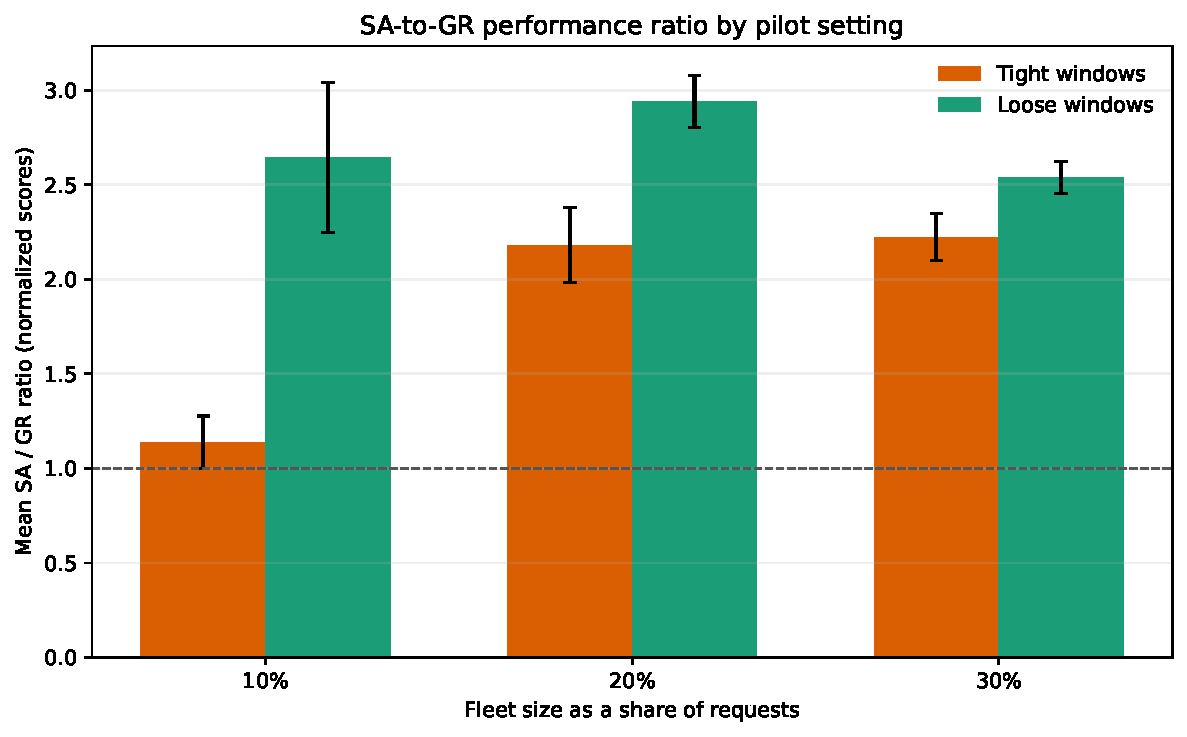
\includegraphics[width=0.78\linewidth]{figures/sa_gr_ratio.pdf}
\caption{Mean SA/GR normalized performance ratio by pilot time-window setting
and fleet size; error bars show one standard deviation across 12 cases in each
group. A ratio above 1 favours SA. Data:
\sourcepath{pilot/work/results/perf_matrix.csv}.}
\end{figure}

The seed issue is documented as 6 distinct \texttt{od\_distance\_mean} values
before the fix and 24 after it. The available pre-fix-labelled file has only
24 rows and 3 distinct values; the other 72-row files have 24. The pre-fix
value of 6 cannot be reproduced from these files, so no before/after bar chart
is shown. The post-fix value of 24 is present in
\sourcepath{pilot/work/results/features.csv}.

\subsection{Model checker and exact model}

The checker compared the original and rewritten models with the heuristic
feasibility rules in 11 scenarios. The original model mismatched in 9; v2
mismatched in none. The documented v1 defects were construction infeasibility,
capacity effectively \texttt{C-2}, shifted travel-time columns, no third-party
option, and an objective inconsistent with the heuristic.

\begin{table}[H]
\centering
\small
\caption{Exact model v2 on small instances. First-run values are from the
available raw record before valid ride lower bounds and other improvements.
Rerun figures are reported by session in \sourcepath{docs/02_tests_and_results.md};
the rerun objective and bound were not tabulated there.}
\begin{tabularx}{\linewidth}{@{}l l r r r r X@{}}
\toprule
Requests & Run & Objective & Bound & Gap & Time (s) & Result\\
\midrule
5 & First & 7284.99 & 170.376 & 97.66\% & 3600.02 & Time limit\\
5 & Rerun & Not tabulated & Not tabulated & 0\% (optimal) & 2.5 & Optimal after valid ride lower bounds\\
10 & First & 16261 & 0 & 100\% & 3600.07 & Time limit\\
10 & Rerun & Not tabulated & Not tabulated & 25\% & 3600 limit & Gap reported at limit\\
15 & First & 39034 & 0 & 100\% & 3600.35 & Time limit\\
15 & Rerun & Not tabulated & Not tabulated & Not reported & 3600 limit & Not solved to optimality\\
\bottomrule
\end{tabularx}
\end{table}

\noindent\textit{Table note:} Rerun status, gap, and five-request time are
reported by session; no rerun raw log is identified in the source. First-run
objective, bound, gap, and time are transcribed from
\sourcepath{pilot/work/v2_tests/v2_results.txt}. The \SI{3600}{s} rerun limits
for 10 and 15 requests follow the documented one-hour limit; a precise
termination time is not given. SA was reported as 4.6\% above v2's proven
five-request optimum and at least 20\% above the unproven ten-request v2
solution. A full SA/v2 objective-and-vehicle table is \tagopen[A5].

\subsection{Generation profile}

The six-request profile took 250 seconds wall time and 192 seconds CPU before
the cache. Nearest-node lookup accumulated 117.8 seconds of the 154.3-second
request phase; imports took about 60 seconds and the request plot about
27 seconds. After the fix, the whole run took 115 seconds wall time and 72
seconds CPU. The reported post-fix maximum memory of 67 MB is suspicious and
must not be used for sizing \tagopen[G6].

\begin{figure}[H]
\centering
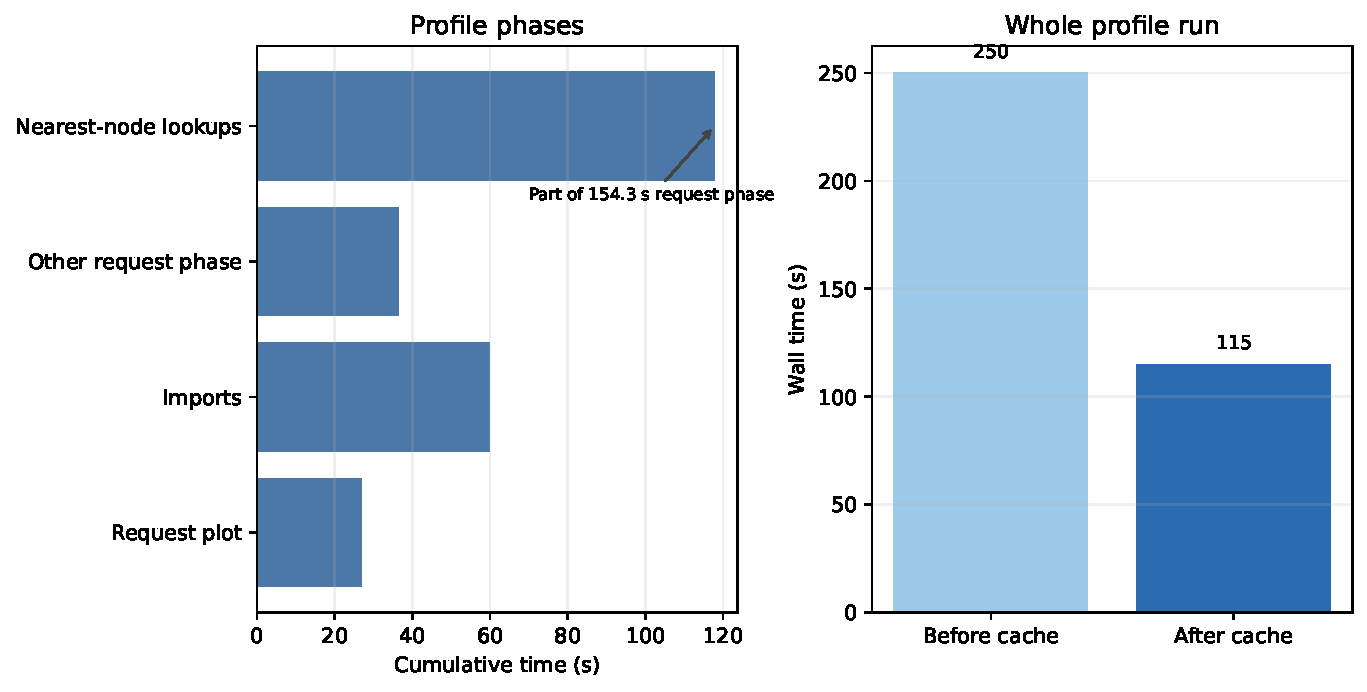
\includegraphics[width=0.78\linewidth]{figures/generation_profile.pdf}
\caption{Measured generation costs before the nearest-node cache and total
wall time before/after it. The nearest-node bar is part of the full request
phase, not an additional phase. After-fix total uses the documented 115 s
measurement. Source: \sourcepath{docs/02_tests_and_results.md}, T7.}
\end{figure}

\subsection{Network build and resource use}

The region network contains 3515 stations, with none on Bornholm. The build
used one core and ran for 3.4 hours while waiting on Overpass for part of the
time. A separate generation job with a station matrix had used 7.1 GB of an
8 GB reservation after 5.3 hours and had written no output files. The eventual
job result is \tagopen[G1]; the unaccounted time is \tagopen[G3].

\begin{table}[H]
\centering
\small
\caption{Recorded HPC resource use. Reserved memory is per slot. Missing or
unmeasured values are marked rather than estimated.}
\begin{tabularx}{\linewidth}{@{}p{0.20\linewidth}p{0.10\linewidth}p{0.14\linewidth}p{0.12\linewidth}p{0.15\linewidth}p{0.14\linewidth}@{}}
\toprule
Phase & Cores & Reserved & Used & CPU use & Runtime\\
\midrule
Network build & 1 & 6 GB & 4466 MB & 28\% & 12374 s (3.4 h)\\
6-request profile, before fix & 1 & 8 GB & 1593 MB & 77\% & 250 s\\
6-request profile, after fix & 1 & 8 GB & 67 MB\textsuperscript{a} & 63\% & 115 s\\
218-request generation test & 1 & 8 GB & 7.1 GB & About 1 core & 5.3 h, unfinished\\
SA/GR pilot solver & 1 & 16 GB & About 6 GB & Not reported & Not reported\\
Exact model v2 & 4 threads\textsuperscript{b} & Not stated & Not stated & Not stated & 1 h limit\\
\bottomrule
\end{tabularx}
\end{table}

\noindent\textsuperscript{a}The 67 MB maximum is identified as suspicious in the
source. \textsuperscript{b}The first-run raw logs show four threads; the HPC
resource table says the exact-model resource size is not yet established.
The exact-model rerun status and timing are reported by session. For network
and profile measurements, values are transcribed from the documented
measurements; the raw session logs are not all identified. Do not treat
unreported solver CPU use or runtime as zero.

\section{Decisions log}

\begin{longtable}{@{}p{0.08\linewidth}p{0.84\linewidth}@{}}
\caption{Short form of the decisions recorded in \sourcepath{docs/01_decisions.md}.}\\
\toprule
ID & Decision\\
\midrule
\endfirsthead
\toprule
ID & Decision\\
\midrule
\endhead
D1 & Optimise passenger ride time plus a four-times direct-time penalty for third-party service; operator cost is post hoc.\\
D2 & Use SA and GR in the ISA performance matrix; use exact Gurobi only for validation on 5--15 requests.\\
D3 & A third ISA algorithm is wanted, but its exact variant is \tagopen.\\
D4 & Use the matheuristic to identify where SA is weak, not as an ISA algorithm.\\
D5 & Use the Capital Region of Denmark without Bornholm.\\
D6 & Use a two-hour period starting 12:00--19:30.\\
D7 & Use 50--500 requests per hour (100--1000 per instance).\\
D8 & Draw continuous settings with Latin hypercubes, not a small factorial grid.\\
D9 & Grow the set in batches until space growth is small or a cap is reached.\\
D10 & Do not vary depots or hotspots during generation; choose the depot later.\\
D11 & Draw three fleets per request instance with a second Latin hypercube.\\
D12 & Use the documented walking, vehicle-speed, and direct-trip-time settings.\\
D13 & Write the shared station travel-time matrix once per network.\\
D14a & Keep the current request range for now; it may be raised later.\\
D14b & Compute the station matrix in a separate HPC job.\\
D14 & Keep settings editable in \sourcepath{isa_set/design.json}; final choices belong to the author.\\
D15 & Replace the earlier IP model with model v2.\\
D16 & Make request seeds depend on the config seed.\\
D17 & Restrict station, school, and hospital lookups to the network polygon.\\
D18 & Use a cached nearest-node index in request sampling.\\
D19 & Preserve directed travel times and convert walking distance to seconds.\\
D20 & Keep hybrid-feasibility code but deprecate it for this ISA.\\
D21 & Run solvers and long generation jobs on DTU HPC, not the author's PC.\\
D22 & Reserve only measured resources with modest headroom; report CPU, wall time, and maximum memory.\\
\bottomrule
\end{longtable}

\section{Open questions and next steps}

The table consolidates every open item in the source notes. Repeated mentions
of the same issue (for example the station-matrix cost in the test results and
the open-items list) appear once. Items marked done in the notes are not
relisted as open.

\begin{longtable}{@{}p{0.12\linewidth}p{0.58\linewidth}p{0.17\linewidth}@{}}
\caption{Open items and whether they block the full set or a later analysis.}\\
\toprule
ID & Item & Blocking?\\
\midrule
\endfirsthead
\toprule
ID & Item & Blocking?\\
\midrule
\endhead
\textbf{OPEN-G1} & Determine the final result of test job 29846018; it reached the six-hour limit with no output files. & Yes: full generation\\
\textbf{OPEN-G3} & Measure where the test job's unaccounted \(\sim\)4 hours went; run the separate station-matrix job and record time and memory. & Yes: full generation\\
\textbf{OPEN-G4} & Implement the feature step that attaches the shared station matrix, required for consistent time-window features. & Yes: feature pipeline\\
\textbf{OPEN-G5} & Choose batch memory and wall-time settings from a measured full instance. & Yes: batch runs\\
\textbf{OPEN-G6} & Resolve the suspicious 67 MB maximum-memory report after the nearest-node fix; do not size from it. & No: verify before sizing\\
\textbf{OPEN-A1} & Choose the third ISA algorithm (SA configuration or max-ALNS) and identify its code. & No: ISA algorithm set\\
\textbf{OPEN-A2} & Run the MIP-based matheuristic on HPC and record results. & No: matheuristic study\\
\textbf{OPEN-A3} & Resize SA/GR memory reservation (16 GB reserved; about 6 GB used). & No: solver efficiency\\
\textbf{OPEN-A4} & Commit and rebuild the solver with \texttt{maxstations} 4000. & Yes: Capital Region solver run\\
\textbf{OPEN-A5} & Tabulate SA and v2 objectives, bounds, and vehicles used on the 5- and 10-request cases. & No: validation report\\
\textbf{OPEN-A6} & Test whether SA's 70-of-72 advantage over GR persists on the wide design. & No: full-set analysis\\
\textbf{OPEN-S1} & Revisit the request range if generation cost allows going above 50--500 per hour; the current range is decided for now. & No: later design revision\\
\textbf{OPEN-S2} & Decide whether maximum walking time should vary, given its effect on candidate stops. & No: design choice\\
\textbf{OPEN-S3} & Decide whether several depots affect algorithm-performance differences. & No: design choice\\
\textbf{OPEN-S4} & Set the cap for batches of 100 instances. & Yes: stopping rule\\
\textbf{OPEN-D1} & Add a description of what \sourcepath{REQreate/rank_model.py} computes. & No: documentation\\
\textbf{OPEN-D2} & Diagnose or document the seven web-app tests that fail on this branch and its predecessor. & No: unrelated test suite\\
\textbf{OPEN-D3} & Determine why the first generation job-array attempt passed an empty config argument. & No: replaced workflow\\
\textbf{OPEN-D4} & Clarify that the \sourcepath{/jobs} reminder tracks only assistant-run \texttt{bsub} commands. & No: monitoring\\
\textbf{OPEN-T3} & Establish resource sizing for the exact-model jobs; the source lists threads and memory as not yet sized. & No: exact-model scale-up\\
\bottomrule
\end{longtable}

The same next-step priorities follow from the evidence: complete and measure
the station-matrix path before scaling generation; resolve memory reports
before setting reservations; then expand the instance set and test algorithm
selection on the continuous design. The author still makes final choices for
the \tagprop settings.

\section{Reproduction}

The full generation and solver pipeline is intended for DTU HPC. These commands
are transcribed from \sourcepath{docs/05_hpc_and_reproduction.md}; they are
not to be run as local solver or generation jobs.

\begin{lstlisting}[language=bash]
# Build the network once
bash ~/instance-generator/isa-features-plan-implementation/isa_set/hpc/build_network.sh

# Draw a batch of 100, then submit one single-core job per config
python ~/instance-generator/isa-features-plan-implementation/isa_set/make_batch.py --batch 1 --n 100
bash ~/instance-generator/isa-features-plan-implementation/isa_set/hpc/generate_batch.sh 1

# Profile a small generation run
bsub -J isa_prof -q hpc -n 1 -R "rusage[mem=8GB]" -M 8GB -W 1:00 \
  -o /work3/$USER/isa/logs/profile.out \
  bash ~/instance-generator/isa-features-plan-implementation/isa_set/hpc/profile_one.sh <config.json> 6
\end{lstlisting}

\noindent\texttt{MEM\_GB} and \texttt{WALL\_H} override the 8 GB and 6 hour
generation defaults. The recorded log pattern is
\sourcepath{/work3/<user>/isa/logs/batch_XX/gen_<instance>.out}. The documented
pipeline then collects feature rows, runs SA and GR for every instance/fleet,
projects the set with \sourcepath{src/isa_pipeline.py}, and measures space
growth. The matrix attachment step needed for the time-window features is not
written yet \tagopen[G4].

\section{Source and verification notes}

\subsection{Figures and their data sources}

\begin{itemize}
\item \textbf{Figure 1, pilot instance space:}
  \sourcepath{pilot/work/results/instance_space.csv} and
  \sourcepath{pilot/work/results/perf_matrix.csv}.
\item \textbf{Figure 2, SA/GR ratio by fleet and time window:}
  \sourcepath{pilot/work/results/perf_matrix.csv}.
\item \textbf{Figure 3, generation profile:}
  measured values in \sourcepath{docs/02_tests_and_results.md}, T7. The
  after-fix total wall-time bar is from the measured 115-second rerun. There is
  no source CSV for the profile timings.
\end{itemize}

All three PDFs are regenerated by \sourcepath{make_figures.py}. The seed-count
comparison is intentionally text-only because the available pre-fix data do
not reproduce the documented value.

\subsection{Numbers not independently verified from raw records}

\begin{itemize}
\item The pre-fix count of 6 distinct \texttt{od\_distance\_mean} values is
  reported in the docs but not reproduced by the available data. The available
  pre-fix-labelled CSV has 24 rows and 3 distinct values; the post-fix files
  have 24 distinct values.
\item The rerun exact-model result (5 requests optimal in 2.5 s, 10 requests
  at 25\% gap, and 15 requests not optimal) is reported by session. The source
  does not identify a raw rerun log, nor tabulate rerun objectives or bounds.
\item The 67 MB post-fix maximum-memory result is expressly described as
  suspicious in the source and is not a reliable memory estimate.
\item The final outcome of generation job 29846018, the measured station-matrix
  time and memory, the cause of the extra generation time, and resource sizes
  for subsequent batches are not available.
\item The exact-model objectives and bounds for the rerun, and the comparative
  SA/v2 vehicle-use table, remain unreported.
\end{itemize}

\subsection{Source inconsistencies to resolve}

\begin{itemize}
\item The feature list gives general request-count ranges of 5000--20000 and
  fleet-size ranges of 15--25\%; the current study design instead uses
  100--1000 requests per instance and 5--40\% fleet size. The study-specific
  design is taken from \sourcepath{isa_set/design.json}, but the older feature
  range should be reconciled in the source notes.
\item The paper-settings file describes the pilot period as 6:30--8:30, while
  the generator-change notes describe pilot v2 as having a real 7:30 peak and
  the current design as low-demand starts between 12:00 and 19:30. These may
  refer to different protocol versions; the source set does not fully explain
  the difference.
\item The docs report six pre-fix distinct mean OD distances over 72 pilot
  cases, but available \sourcepath{pilot/work/pilot_v1/results/features.csv}
  contains 24 rows and 3 distinct values. The 72-row files labelled
  \sourcepath{pilot_v2_old} and \sourcepath{results} each contain 24 distinct
  values. The files therefore do not reproduce the stated before-fix/after-fix
  comparison as described.
\item The design JSON names the network as the Capital Region but does not
  encode the Bornholm exclusion in the network string. The decisions and
  network test specify the exclusion, so it is treated as part of the design
  here.
\end{itemize}


\bibliographystyle{plain}
\bibliography{references}
\end{document}
